\subsubsection{Example 1: The Heat Equation}
    \begin{example}[CG-DG-in-time discretization for the heat equation]
        Consider the heat equation (\ref{eqn:heat equation}) on $\bfOmega\otimes T$ for $T  =  \left(0, t^{N}\right]$, with homogeneous Dirichlet/Neumann boundary conditions, such that in the strong form, the dissipation equation (\ref{eqn:heat equation dissipation}) holds. Suppose further the initial conditions (ICs) at $t  =  0$, $u  =  \widehat{u}_{0}|_{t = 0}$ hold.
        
        To cast into a chosen weak form in time, define:
        \begin{itemize}
            \item  A test space $\calU$, with $\calU_{-}  :=  \{u  \in  \calU  : 
         u|_{t = 0}  =  0\}$
            \item  A trial space $\calV$
        \end{itemize}
        supported on $\bfOmega\otimes T$. One seeks $u_{-}  \in  \calU_{-}$ such that $\forall  v  \in  \calV$,
        \begin{equation}\label{eqn:heat equation weak form}
            \langle v, \partial_{t}u\rangle_{\bfOmega\otimes T}  =   - \frac{1}{\rmPe}\langle\nabla v, \nabla u\rangle_{\bfOmega\otimes T},
        \end{equation}
        where, to incorporate the ICs, $u$ is $u_{-}$ with a lifting of the ICs, $u  :=  u_{0} + u_{-}$, where in turn $u_{0}  \in  \calU$ is an extension of the ICs to be supported on $\bfOmega\otimes T$.
        
        To create an order-$s$ CG-DG FET timestepper, define:
        \begin{align}
            \bbU^{h}  :=  \widehat{\calU}(\bfOmega)\otimes\bbP^{s}\left(T^{h}\right)  <  \calU,  &&
            \bbV^{h}  :=  \widehat{\calV}(\bfOmega)\otimes\bbDP^{s - 1}\left(T^{h}\right)  <  \calV,
        \end{align}
        where $T^{h}$ is a mesh of $N$ intervals on $T$, at timesteps $0$, $t^{1}$, $t^{2}$, $\cdots$, with $\bbU^{h}_{-}$ defined analogously to $\calU_{-}$. Mapping $\calU_{-}  \mapsto  \bbU^{h}_{-}$, $\calV_{-}  \mapsto  \bbV^{h}_{-}$ in (\ref{eqn:heat equation weak form}) invokes the Petrov–Galerkin projection. Denote bases for these FE spaces:
        \begin{align}
            (\phi_{j})_{j}     \text{ for }  \bbP^{s}\left(T^{h}\right),         &&
            (\varphi_{i})_{i}  \text{ for }  \bbDP^{s - 1}\left(T^{h}\right).
        \end{align}
        $u^{h}  \in  \bbU^{h}$, $v^{h}  \in  \bbV^{h}$ can be expressed in terms of these bases as:
        \begin{align}
            u^{h}(\bfx; t)  =  \sum_{j}\widehat{u}_{j}(\bfx)\phi_{j}(t),  &&
            v^{h}(\bfx; t)  =  \sum_{i}\widehat{v}_{i}(\bfx)\varphi_{i}(t)
        \end{align}
        for $\left(\widehat{u}_{j}\right)_{j}$ in $\widehat{\calU}$, $\left(\widehat{v}_{i}\right)_{i}$ in $\widehat{\calV}$. The Petrov–Galerkin-projected weak form then states that, $\forall  \left(\widehat{v}_{i}\right)_{i}$ in $\widehat{\calV}$:
        \begin{align}
            \left\langle\sum_{i}\widehat{v}_{i}\varphi_{i}, \partial_{t}\left[\sum_{j}\widehat{u}_{j}\phi_{j}\right]\right\rangle_{\bfOmega\otimes T^{h}}  &=  - \frac{1}{\rmPe}\left\langle\nabla\left[\sum_{i}\widehat{v}_{i}\varphi_{i}\right], \nabla\left[\sum_{j}\widehat{u}_{j}\phi_{j}\right]\right\rangle_{\bfOmega\otimes T^{h}}  \\
            \sum_{i, j}\left\langle\widehat{v}_{i}, \widehat{u}_{j}\right\rangle_{\bfOmega}\langle\varphi_{i}, \partial_{t}\phi_{j}\rangle_{T^{h}}  &=  - \frac{1}{\rmPe}\sum_{i, j}\left\langle\nabla\widehat{v}_{i}, \nabla\widehat{u}_{j}\right\rangle_{\bfOmega}\langle\varphi_{i}, \phi_{j}\rangle_{T^{h}}
        \end{align}
        Denoting the vectors $\widehat{\bfu}  :=  \left(\widehat{u}_{j}\right)_{j}$, $\widehat{\bfv}  :=  \left(\widehat{v}_{i}\right)_{i}$, and mass and stiffness bilinear operators $\calM\left[\widehat{v}, \widehat{u}\right]  :=  \left\langle\widehat{v}, \widehat{u}\right\rangle_{\bfOmega}$, $\calK\left[\widehat{v}, \widehat{u}\right]  :=  \left\langle\nabla\widehat{v}, \nabla\widehat{u}\right\rangle_{\bfOmega}$ respectively, this takes the matrix form, $\forall  \widehat{\bfv}  \in  \widehat{\calV}^{Ns}$:
        \begin{align}
            \widehat{\bfv}^{\rmT}(\langle\varphi_{i}, \partial_{t}\phi_{j}\rangle_{T^{h}}\calM)^{j}_{i}\widehat{\bfu}  =  - \frac{1}{\rmPe}\widehat{\bfv}^{\rmT}(\langle\varphi_{i}, \phi_{j}\rangle_{T^{h}}\calK)^{j}_{i}\widehat{\bfu}  \\
            \widehat{\bfv}^{\rmT}\left(\langle\varphi_{i}, \partial_{t}\phi_{j}\rangle_{T^{h}}\calM + \frac{1}{\rmPe}\langle\varphi_{i}, \phi_{j}\rangle_{T^{h}}\calK\right)^{j}_{i}\widehat{\bfu}  =  0
        \end{align}
        
        Regarding the sparsity of this matrix, with appropriate ordering of the bases $(\phi_{i})_{i}$, $(\varphi_{i})_{i}$, the matrices $(\langle\varphi_{i}, \partial_{t}\phi_{j}\rangle_{T^{h}})^{j}_{i}$, $(\langle\varphi_{i}, \phi_{j}\rangle_{T^{h}})^{j}_{i}$ take the general form
        \begin{equation}\label{eqn:timestepper matrices}
            \left(\begin{array}{ c : c c : c c : c c }
                \pm\bfb  &  \bfA    &  \bfb     &  0       &  0        &  \cdots   &  0        \\
                \hdashline
                0        &  0       &  \pm\bfb  &  \bfA    &  \bfb     &  \cdots   &  0        \\
                \hdashline
                0        &  0       &  0        &  0       &  \pm\bfb  &  \cdots   &  0        \\
                \hdashline
                \vdots   &  \vdots  &  \vdots   &  \vdots  &  \vdots   &  \ddots   &  \vdots   \\
                \hdashline
                0        &  0       &  0        &  0       &  0        &  \cdots   &  \bfb     \\
            \end{array}\right)
        \end{equation}
        for some $\bfA  \in  \bbR^{s\times (s - 1)}$, $\bfb  \in  \bbR^{s}$ in either case, dependent on the choice of bases. (See Figure \ref{fig:timestepper matrices})
        
        \begin{figure}[!ht]
            \centering
            \begin{subfigure}{0.5\textwidth}
                \centering
                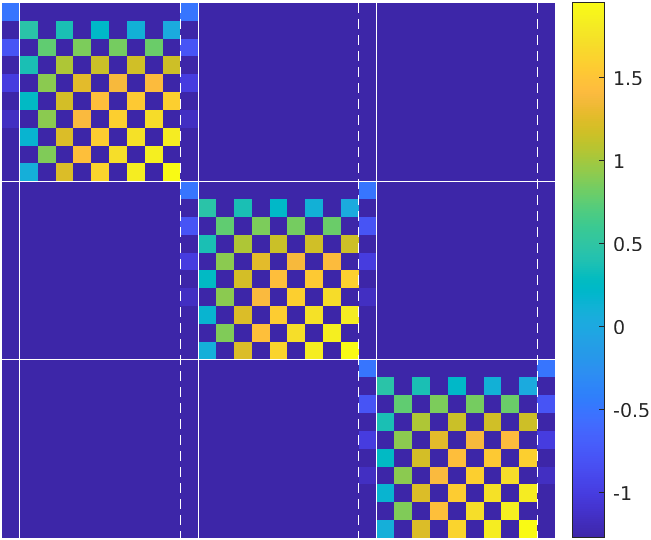
\includegraphics[width = 0.9\textwidth]{9 - finite elements in time/images/matrix 1.png}
                \caption{$(\langle\varphi_{i}, \partial_{t}\phi_{j}\rangle_{T^{h}})^{j}_{i}$}
            \end{subfigure}%
            \begin{subfigure}{0.5\textwidth}
                \centering
                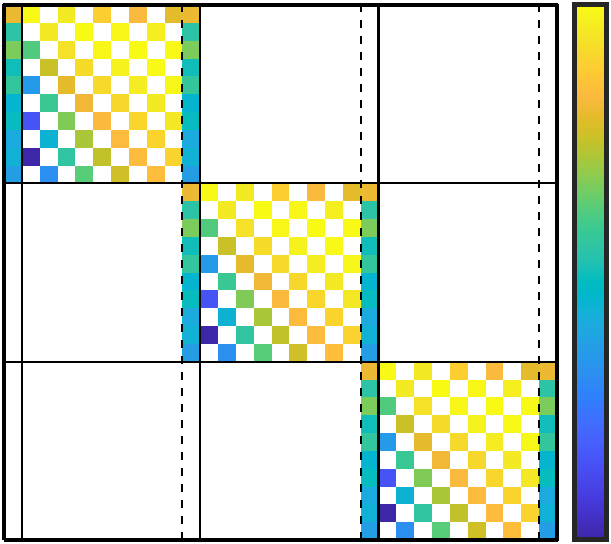
\includegraphics[width = 0.9\textwidth]{9 - finite elements in time/images/matrix 2.png}
                \caption{$(\langle\varphi_{i}, \phi_{j}\rangle_{T^{h}})^{j}_{i}$}
            \end{subfigure}
            \caption{Sparsity plots for the two timestepping matrices when $s  =  10$ on $(N  =)  3$ (equal) intervals, under simple normalised polynomial bases. \\ Color indicates $\log(|*|)$ for the matrix entries. Black lines indicate block structure from (\ref{eqn:timestepper matrices}), while solid black lines highlight the lower-block-triangular structure after elimination of first column on restriction of $\bbU^{h}  \mapsto  \bbU^{h}_{-}$ with the strong enforcement of the ICs.}
            \label{fig:timestepper matrices}
        \end{figure}
        
        Restricting $\bbU^{h}  \mapsto  \bbU^{h}_{-}$ with the strongly imposition of the ICs, the first column of this matrix is eliminated, since $\phi_{0}$ is eliminated from the basis in time, leaving a lower-block-triangular matrix composed of size-$p$ blocks. This is indicated by the dashed lines in (\ref{eqn:timestepper matrices}). 
        
        Applying block forward substitution to solve this block-triangular problem is then perfectly analogous to using a traditional timestepper. On the $n$-th timestep, $\forall  \left(\widehat{v}_{ns + i}\right)_{i = 1, \cdots, s}$ in $\widehat{\calV}$:
        \begin{equation}
            \sum_{\begin{smallmatrix}  i = 1, \cdots, s  \\  j = 0, \cdots, s  \end{smallmatrix}}\left\langle\widehat{v}_{ns + i}, \widehat{u}_{ns + j}\right\rangle_{\bfOmega}\langle\varphi_{ns + i}, \partial_{t}\phi_{ns + j}\rangle_{T^{h}}  =  - \frac{1}{\rmPe}\sum_{\begin{smallmatrix}  i = 1, \cdots, s  \\  j = 0, \cdots, s  \end{smallmatrix}}\left\langle\nabla\widehat{v}_{ns + i}, \nabla\widehat{u}_{ns + j}\right\rangle_{\bfOmega}\langle\varphi_{ns + i}, \phi_{ns + j}\rangle_{T^{h}}
        \end{equation}
        \begin{multline}
            \sum_{\begin{smallmatrix}  i = 1, \cdots, s  \\  j = 1, \cdots, s  \end{smallmatrix}}\left(\left\langle\widehat{v}_{ns + i}, \widehat{u}_{ns + j}\right\rangle_{\bfOmega}\langle\varphi_{ns + i}, \partial_{t}\phi_{ns + j}\rangle_{T^{h}} + \frac{1}{\rmPe}\left\langle\nabla\widehat{v}_{ns + i}, \nabla\widehat{u}_{ns + j}\right\rangle_{\bfOmega}\langle\varphi_{ns + i}, \phi_{ns + j}\rangle_{T^{h}}\right)  \\
            =  - \sum_{i = 1, \cdots, s}\left(\left\langle\widehat{v}_{ns + i}, \widehat{u}_{ns}\right\rangle_{\bfOmega}\langle\varphi_{ns + i}, \partial_{t}\phi_{ns}\rangle_{T^{h}} + \frac{1}{\rmPe}\left\langle\nabla\widehat{v}_{ns + i}, \nabla\widehat{u}_{ns}\right\rangle_{\bfOmega}\langle\varphi_{ns + i}, \phi_{ns}\rangle_{T^{h}}\right)
        \end{multline}
        which can be solved iteratively for each $\bfu_{(n + 1)s}$ at each new timestep.

        In the case of $s  =  1$—the lowest-order method—with time intervals of length $\delta t^{n} 
         =  t^{n + 1} - t^{n}$, this takes the form, $\forall \widehat{v}_{n}  \in  \widehat{\calV}$,
        \begin{equation}
            \left\langle\widehat{v}_{n + 1}, \widehat{u}_{n + 1}\right\rangle_{\bfOmega} + \frac{\delta t^{n}}{2\rmPe}\left\langle\nabla\widehat{v}_{n + 1}, \nabla\widehat{u}_{n + 1}\right\rangle_{\bfOmega}  =  \left\langle\widehat{v}_{n + 1}, \widehat{u}_{n + 1}\right\rangle_{\bfOmega} - \frac{\delta t^{n}}{2\rmPe}\left\langle\nabla\widehat{v}_{n + 1}, \nabla\widehat{u}_{n}\right\rangle_{\bfOmega},
        \end{equation}
        which, by rearranging, can be seen to be equivalent to the traditional implicit midpoint method,
        \begin{equation}
            \left\langle\widehat{v}_{n + 1}, \frac{1}{\delta t}\left(\widehat{u}_{n + 1} - \widehat{u}_{n}\right)\right\rangle_{\bfOmega}  =  - \frac{1}{\rmPe}\left\langle\nabla\widehat{v}_{n + 1}, \frac{1}{2}\nabla\left(\widehat{u}_{n + 1} + \widehat{u}_{n}\right)\right\rangle_{\bfOmega}.
        \end{equation}
        For $s  >  1$—at higher order—the resultant timesteppers are equivalent to the higher-order GL methods, which are known to be exactly dissipative for the heat equation.
    \end{example}